
\documentclass[a4paper]{article}
\usepackage[fontset=fandol]{ctex}
\usepackage{amsmath, amssymb}
\usepackage{graphicx}
\usepackage[margin=2.3cm]{geometry}
\usepackage[most]{tcolorbox}
\usepackage{listings}
\usepackage{hyperref}
\usepackage{booktabs}
\usepackage{float}
\usepackage{xcolor}

\lstset{
    basicstyle=\ttfamily\small,
    breaklines=true,
    frame=single,
    numbers=left,
    numberstyle=\tiny\color{gray}
}

\newtcolorbox{knowledgebox}[1]{
    enhanced,
    colback=blue!5!white,
    colframe=blue!70!black,
    colbacktitle=blue!70!black,
    coltitle=white,
    fonttitle=\bfseries,
    title=#1,
    sharp corners
}

\newtcolorbox{importantbox}[1]{
    enhanced,
    colback=yellow!10!white,
    colframe=yellow!70!black,
    colbacktitle=yellow!70!black,
    coltitle=black,
    fonttitle=\bfseries,
    title=#1,
    sharp corners
}

\newtcolorbox{warningbox}[1]{
    enhanced,
    colback=red!5!white,
    colframe=red!70!black,
    colbacktitle=red!70!black,
    coltitle=white,
    fonttitle=\bfseries,
    title=#1,
    sharp corners
}

\begin{document}

\begin{titlepage}
\centering
{\Large 课程讲义\par}
\vspace{1.2cm}
{\huge\bfseries Advanced topics in theorem proving\par}
\vspace{0.4cm}
{\Large CS294/194-280: Advanced Large Language Model Agents\par}
\vspace{0.4cm}
{\large Sean Welleck, Carnegie Mellon University\par}
\vspace{0.4cm}
{\large 中文教材化讲义 / Harness Build\par}
\vspace{0.8cm}
\includegraphics[width=0.84\textwidth,height=0.38\textheight,keepaspectratio]{cover.jpg}\par
\vfill
\begin{tcolorbox}[width=0.92\textwidth,colback=black!2!white,colframe=black!60,sharp corners]
\textbf{课程页}：\href{https://rdi.berkeley.edu/adv-llm-agents/sp25}{https://rdi.berkeley.edu/adv-llm-agents/sp25}\par
\textbf{录播}：\href{https://www.youtube.com/live/Gy5Nm17l9oo}{https://www.youtube.com/live/Gy5Nm17l9oo}\par
\textbf{Slides}：\href{https://rdi.berkeley.edu/adv-llm-agents/slides/welleck2025_berkeley_bridging.pdf}{welleck2025\_berkeley\_bridging.pdf}\par
\textbf{补充 readings}：DSP / miniCTX / Lean-STaR / ImProver
\end{tcolorbox}
\end{titlepage}

\tableofcontents
\newpage

\section{本讲学习目标}

这一讲把课程从 ``agent 会不会推理'' 推向 ``agent 能否在 proof assistant 中稳定地产生、指导、改写与扩展证明''。读完本章后，读者应当能够回答：
\begin{itemize}
\item 为什么 theorem proving 对 agent 研究是高价值场景：它既需要复杂 reasoning，又提供了机器可检验的反馈。
\item 什么是 informal mathematics、formal mathematics，以及它们之间的 \textbf{非形式到形式鸿沟（informal-formal gap）}。
\item Lean-STaR 如何把 \textbf{思考（thought）} 显式插入 tactic prediction 之前，并利用成功 proof 做 expert iteration。
\item Draft, Sketch, Prove 为什么不是把自然语言证明直接当答案，而是把它当成 formal search 的结构偏置。
\item LeanHammer 与 miniCTX 分别解决 theorem proving 里的哪一类瓶颈：一个偏低层自动证明与 premise selection，一个偏 research-level 长上下文依赖。
\item ``证明已经正确'' 与 ``证明已经优化'' 是两个不同问题；proof optimization 为什么会成为 agent 化的新任务。
\end{itemize}

\section{背景与问题设置}

\subsection{为什么数学证明是 agent 的理想试验场}

Sean Welleck 一开场先把数学放进 expert-domain agent 的谱系里：金融、医疗、数学都属于错误代价高、需要结构化 reasoning、又必须能解释中间过程的领域。与开放式对话不同，数学和形式验证的好处是：系统可以把问题写成 specification，把候选解写成 proof code，再让 proof assistant 做严格检查。这样一来，agent 并不是只在 ``像不像合理回答'' 的层面被评估，而是能收到 \textbf{编译是否通过、哪一步失败、缺了哪些前提} 这样的环境反馈。

\subsection{informal mathematics 与 formal mathematics 的区别}

讲座先对两类数学对象做了清晰区分。所谓 \textbf{非形式数学（informal mathematics）}，是论文、教材、草稿、板书、图示和自然语言讨论中的数学。这些材料灵活、可读、便于交流，但通常难以被自动校验。所谓 \textbf{形式数学（formal mathematics）}，则更像 source code：命题需要写成精确 specification，证明需要写成 proof script 或 tactic trace，只要 proof assistant 接受，正确性就获得了机器层面的保证。

\begin{figure}[H]
\centering
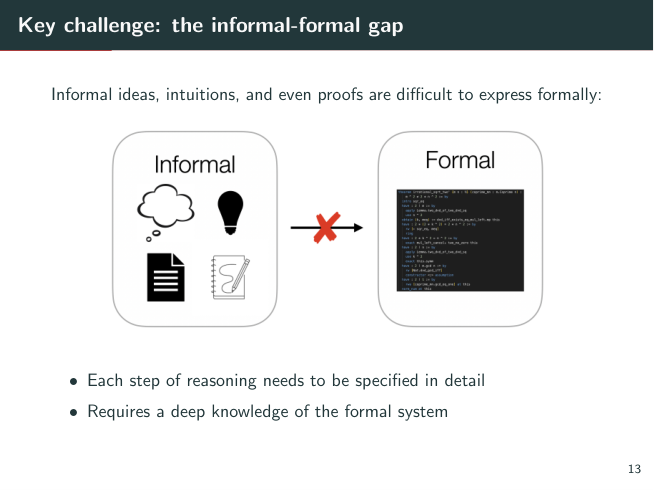
\includegraphics[width=0.82\textwidth]{figures/lec10_fig_001.png}
\caption{informal-formal gap：自然语言中的证明直觉并不会自动变成 proof assistant 能接受的形式对象。}
\end{figure}

这一区分必须和上一讲的 \textbf{autoformalization}、\textbf{theorem proving} 等概念拆开来看。autoformalization 是把自然语言题目或想法翻译成 formal statement；theorem proving 是在 formal statement 已经给定时搜索或构造证明；verification 则是让 proof assistant 或 verifier 检查候选证明的合法性。三者都与数学 reasoning 有关，但承担的角色不同。

\begin{importantbox}{本讲的关键区分}
自然语言 proof sketch 不是 formal proof；formal proof 也不是 theorem discovery。前者提供高层语义结构，后者承担低层可检验正确性，而 discovery 还包括提出 conjecture、定义新对象或发现新规律。
\end{importantbox}

\subsection{为什么 informal-formal gap 是真正瓶颈}

讲座的第一个核心论点是：许多重要数学直觉存在于 informal 层面，例如 ``这里应该做归纳''、``这个量需要先界定一个上界''、``这个证明实际上需要拆成两个子引理''。然而 proof assistant 只理解精细化的 formal state 与 tactic。于是即便一个 LLM 已经在自然语言中 ``知道该怎么做''，它也不一定能把这个想法翻译成逐步可执行的 proof。

这也是 theorem proving 和 L01 中 inference-time reasoning 的深层联系：在普通自然语言任务里，错误往往只在最终答案暴露；在 theorem proving 里，错误会以 type mismatch、missing premise、unsolved goal 等形式被环境立即指出。环境反馈更强，但 search space 也更离散、更脆弱。

\section{从 thought 到 tactic：Lean-STaR}

\subsection{为什么要显式学习 thought}

传统 neural theorem prover 往往直接学习 $p(a_t \mid s_t)$，即给定 proof state 预测下一个 tactic。问题在于，formal proof data 并不记录人类脑中的中间想法。一个数学家写下 tactic 之前，通常已经做了高层判断：当前应该归纳、需要把目标化成某个 lemma、或者先把等式改写成更容易的形式。Lean-STaR 的观察是：如果训练数据只有 tactic，而没有这些 thinking traces，模型学到的只是 ``如何模仿 proof script''，而不是 ``为什么在此刻做这个动作''。

\begin{figure}[H]
\centering
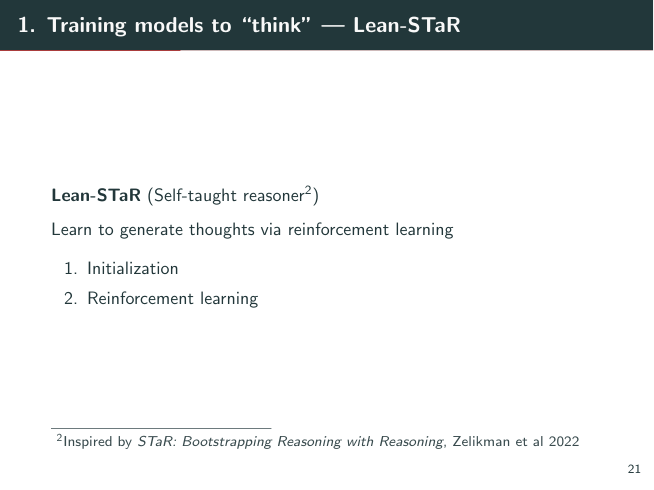
\includegraphics[width=0.76\textwidth]{figures/lec10_fig_002.png}
\caption{Lean-STaR 的结构：在 tactic 之前先生成 informal thought，再把成功证明反过来用于训练 thought+tactic policy。}
\end{figure}

因此，Lean-STaR 把策略改写成 thought 与 tactic 的联合生成：
\[
\pi_{\theta}(z_t, a_t \mid s_t)
\]
其中 $\pi_{\theta}$ 是参数为 $\theta$ 的模型，$s_t$ 是第 $t$ 步 proof state，$z_t$ 是在该步之前生成的 informal thought，$a_t$ 是随后执行的 tactic。这个公式的重要性不在于数学上有多复杂，而在于它明确说：\textbf{推理轨迹本身是策略的一部分，而不是 tactic 的附属注释。}

\paragraph{符号解释}
\begin{itemize}
\item $s_t$：proof assistant 当前暴露给模型的目标、上下文和局部假设。
\item $z_t$：模型对 ``下一步应该怎么想'' 的自然语言或半结构化思考。
\item $a_t$：真正交给 Lean 执行的 tactic。
\item $\pi_{\theta}$：把状态映射到 thought+tactic 联合动作的策略。
\end{itemize}

\subsection{Lean-STaR 的训练与推理循环}

Lean-STaR 并不是人工写 thought annotation，而是从成功 proof 中合成 synthetic thoughts，然后反复自训练。其过程可以概括为：

\begin{lstlisting}
Initialize policy pi_theta(thought, tactic | state)
Collect successful proofs from search
Extract (state, thought, tactic) tuples
Fine-tune the policy on successful tuples
Run search again with the improved policy
\end{lstlisting}

这里的关键有两层。第一，thought 不再是纯 prompt engineering，而是纳入训练目标的显式输出。第二，系统不是一次训练完就结束，而是像 expert iteration 一样，把当前策略能找到的成功 proof 当成下一轮学习的监督信号。这与课程前几讲的 ``verification-backed self-improvement'' 有共通结构：没有 verifier 的反馈，thought 只会变成长篇自言自语；有 verifier 的反馈，thought 才可能变成有效的 search bias。

\subsection{为什么 informal thought 有用}

从本讲 slides 的角度看，thought 至少有三种功能。其一，它帮助模型做 \textbf{状态压缩}：把复杂 proof state 重新描述成高层任务，如 ``此处要做归纳''、``先应用某个对称性 lemma''。其二，它帮助模型做 \textbf{动作筛选}：在 tactic space 非常大时，thought 能把候选动作压缩到语义相关的局部。其三，它帮助模型做 \textbf{预算利用}：当搜索预算增加时，thought 让额外计算不是盲目枚举 tactic，而是沿着更像人类推理的路径展开。

\subsection{实验结果与失败模式}

\begin{figure}[H]
\centering
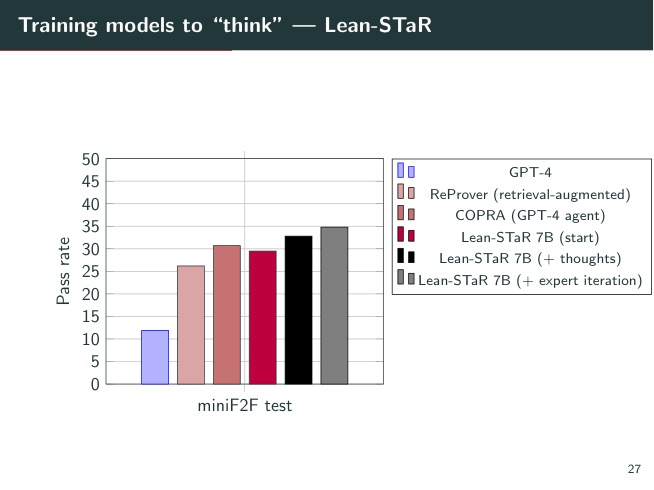
\includegraphics[width=0.78\textwidth]{figures/lec10_fig_003.png}
\caption{Lean-STaR 在 miniF2F 上的结果：thought augmentation 与 expert iteration 都贡献了性能提升。}
\end{figure}

slides 给出的 miniF2F 结果说明：仅仅引入 thoughts 就有帮助，而进一步引入 expert iteration 效果更明显。更关键的是，讲座还强调了一个非常 agent-oriented 的现象：\textbf{随着搜索预算增加，带 thoughts 的系统更能把预算转化为真实通过率。} 这点和 L01 里 ``test-time compute 只有在结构化使用时才有效'' 完全呼应。

\begin{warningbox}{Lean-STaR 不是 free lunch}
thought 本身并不保证正确。若 synthetic thought 质量差、verifier 太弱、search 实现不稳定，模型可能学到看似合理但会误导 tactic 的 explanations。换言之，thought 只是额外中间变量，不是 correctness certificate。
\end{warningbox}

\section{用 informal sketch 指导 formal prover：Draft, Sketch, Prove}

\subsection{高层 reasoning 与低层 proving 的分工}

第二部分的核心是：高层 reasoning 很擅长提出 decomposition、类比和 overall strategy；低层 prover 很擅长做严谨、可验证、细粒度的 proof search。若把两者强行混成同一个黑箱，往往会两头都做不好。Draft, Sketch, Prove（DSP）试图建立一个更清晰的接口：先把 informal theorem 转成 formal theorem，再把 informal proof 变成 formal sketch，最后让 formal prover 在 sketch 引导下完成低层搜索。

\begin{figure}[H]
\centering
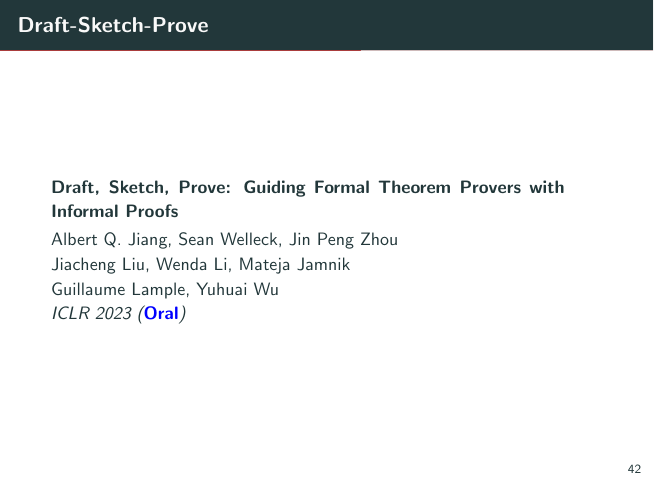
\includegraphics[width=0.78\textwidth]{figures/lec10_fig_004.png}
\caption{DSP 的代表论文页：把 informal theorem 与 informal proof 变成 formal sketch-guided proving 的输入。}
\end{figure}

\subsection{DSP 的形式化视角}

可以把 DSP 理解为在 formal theorem $x_F$ 上引入额外结构约束 $\sigma$：
\[
\tau^{\star} = \arg\max_{\tau \in \mathcal{T}(x_F, \sigma)} r(\tau)
\]
这里 $\tau$ 表示候选 formal proof trajectory，$\mathcal{T}(x_F, \sigma)$ 表示在 theorem $x_F$ 与 sketch $\sigma$ 共同约束下可搜索的 proof 集合，$r(\tau)$ 是 prover 或 verifier 对轨迹的打分，而 $\tau^{\star}$ 是最终选中的证明轨迹。

这条公式传达的直觉非常重要：\textbf{sketch 的价值不是替代搜索，而是重塑搜索空间。} 也就是说，DSP 不是让 LLM 写一段漂亮的自然语言证明然后宣称任务完成，而是把这段高层结构翻译成可操作的约束、子目标或搜索导向。

\subsection{算法流程与小例子}

\begin{lstlisting}
Input informal theorem x_I
Generate a draft formal statement x_F
Produce sketch sigma from informal proof or LLM draft
Guide a low-level prover with sigma
Verify the resulting formal proof in the proof assistant
\end{lstlisting}

若读者想象一个简单例子：自然语言证明可能说 ``先证明集合关系的两个方向，再分别展开定义''。对人来说，这只是常识；对 prover 来说，这相当于巨大 search space 中的关键坐标。DSP 的工作，就是把这种高层提示变成 formal system 能消化的结构化支架。

\subsection{为什么这种方法有效}

slides 中的动机页强调：单纯依赖低层自动证明器时，搜索空间会爆炸，因为系统既要决定整体策略，又要填充每个局部步骤。DSP 通过引入 sketch，把 ``整体路线'' 与 ``局部执行'' 分开，降低了低层 prover 的组合负担。这样做还带来另一个好处：当 informal proof 来自人类或强 LLM 时，系统能直接利用这些高层语义，而不是把它们丢掉再从零 search。

\begin{figure}[H]
\centering
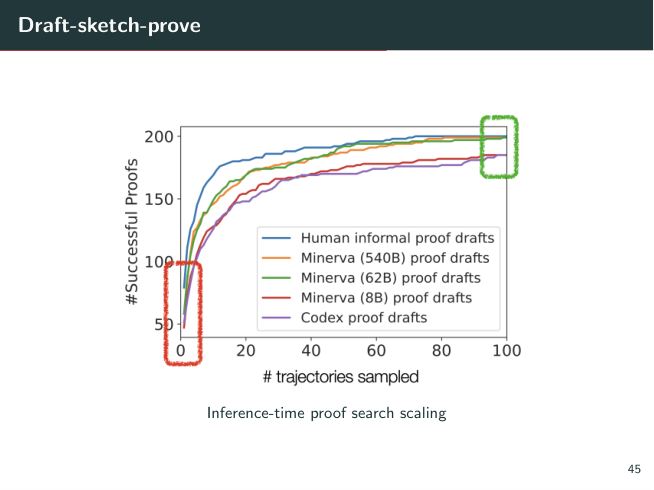
\includegraphics[width=0.76\textwidth]{figures/lec10_fig_005.png}
\caption{DSP 中的 inference-time proof search scaling：好的 sketch 会让额外搜索预算更有效。}
\end{figure}

根据 reading，sketch-guided proving 能把一组竞赛题上的成功率从 20.9\% 提高到 39.3\%。这不是 ``LLM 变得更会证明'' 的简单结论，而更像是：\textbf{当高层结构被显式提供时，低层 formal prover 的效率被显著放大。}

\paragraph{失败模式}
\begin{itemize}
\item 若 draft formal statement 本身错了，后续 proving 会建立在错误目标上。
\item 若 informal proof 太跳跃，sketch 无法映射到稳定子目标。
\item 若低层 prover 无法利用 sketch 提供的信息，系统仍会退化成 brute-force search。
\end{itemize}

\section{LeanHammer：在 Lean 中搭起低层自动证明系统}

\subsection{什么是 hammer}

在 interactive theorem proving 社区，\textbf{hammer} 指的是把外部 automated theorem prover（ATP）接入 proof assistant 的系统。它通常负责 premise selection、格式转换、调用 ATP、再把找到的证明重构回原 proof assistant。Sean Welleck 用 LeanHammer 这一部分强调：如果说 DSP 主要是 ``把 informal reasoning 接进来''，那 hammer 系统关注的就是 ``如何把低层 automation 做强''。

\subsection{premise selection 是低层 proving 的瓶颈}

自动证明器常见的失败原因不是理论上无法证明，而是候选前提太多，搜索分支太广。于是 premise selection 成为核心问题：给定当前 goal $g$ 与上下文 $c$，应该从大规模 library 中挑出哪些 lemmas 或 definitions 送进 ATP？

\[
p^{\star}_{1:k} = \operatorname{TopK}_{p \in \mathcal{P}} f_{\phi}(g, p, c)
\]

这里 $g$ 是当前目标，$p$ 是候选 premise，$\mathcal{P}$ 是可检索的 premise 集，$c$ 是文件或项目上下文，$f_{\phi}$ 是 premise selector 的相关性函数，$p^{\star}_{1:k}$ 是排名靠前、最终送入 ATP 的前 $k$ 个前提。

\paragraph{符号解释}
\begin{itemize}
\item $g$ 决定当前需要证明什么。
\item $c$ 提供额外环境信息，例如当前文件、局部定义、打开的 namespace。
\item $f_{\phi}$ 既可以是稀疏检索，也可以是神经相关性评分器。
\item Top-$k$ 选择体现了 ``先检索，再证明'' 的 agent workflow。
\end{itemize}

\begin{figure}[H]
\centering
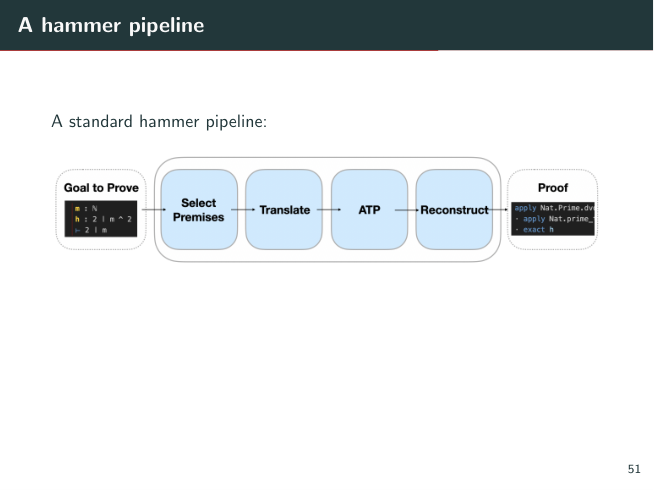
\includegraphics[width=0.82\textwidth]{figures/lec10_fig_006.png}
\caption{标准 hammer pipeline：先做 premise selection，再交给 ATP 与 proof reconstruction。}
\end{figure}

\begin{lstlisting}
Given goal g and context c
Retrieve top-k premises with selector f_phi
Translate the proof state to ATP format
Run ATP and/or tree search
Reconstruct a Lean proof from the successful trace
\end{lstlisting}

\subsection{LeanHammer 为什么比单纯检索更像 agent}

slides 后半段明确展示，LeanHammer 不只是一个 retriever，而是 premise selector、ATP 与 tree search 的组合系统。换句话说，它有感知（读 goal 与上下文）、检索（挑 premise）、行动（调用 prover / tree search）、反馈（proof reconstruction 成败）这几个 agent 环节。

\begin{figure}[H]
\centering
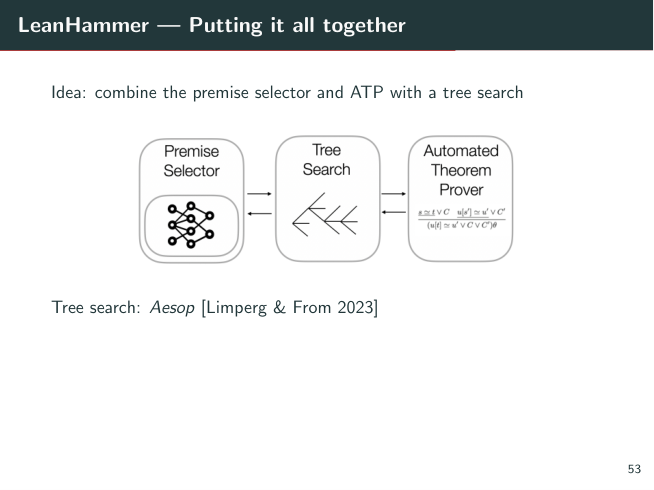
\includegraphics[width=0.78\textwidth]{figures/lec10_fig_007.png}
\caption{LeanHammer 将 premise selector、ATP 与 tree search 组合起来，而不是把它们当成独立模块。}
\end{figure}

这一点和课程前几讲讲到的 workflow agent 很像：好的系统不是只会 ``调用一个工具''，而是知道何时调用哪个工具、失败后如何换轨、以及哪些中间信息要保留给下一轮。LeanHammer 把这些思想放到了 theorem proving 里。

\subsection{量化结果、风险与边界条件}

量化结果页说明，premise selector 的质量直接影响最终 proof rate。即便 ATP 本身很强，如果 premise selection 太差，也会因为无关前提太多而被淹没。反过来，若 premise selection 很准，却缺少可重构证明，系统也无法在 Lean 中落地。

\begin{warningbox}{不要把 hammer 误解为端到端数学推理}
hammer 的强项是把现有 library 和自动证明器用得更好，而不是提出新的 conjecture 或自动完成 research-level 形式化。它解决的是低层 automation bottleneck，不是全部 theorem proving 问题。
\end{warningbox}

\section{research-level formalization 与 miniCTX}

\subsection{为什么竞赛 benchmark 不够}

讲座最后一部分把视角拉到 research-level mathematics。slides 用 Terence Tao 的 blueprint 形式化项目作例子，强调真实数学项目往往跨文件、跨定义、跨引理地组织。这里的瓶颈不再只是单个 theorem 难不难，而是 \textbf{一个项目里哪些上下文真正相关、如何让使用者和模型都能进入该项目语境}。

\begin{figure}[H]
\centering
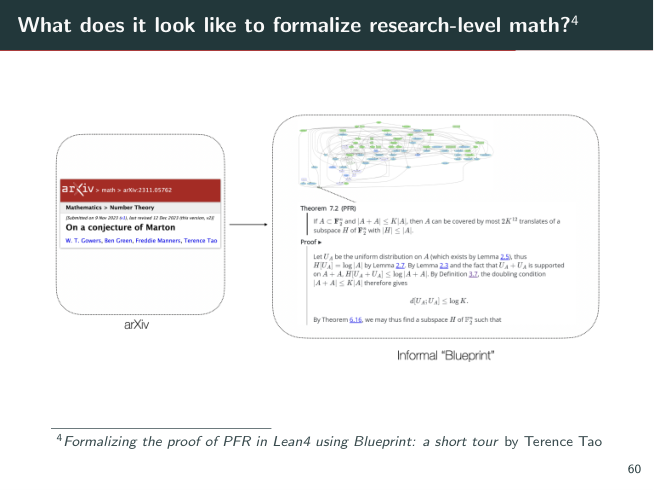
\includegraphics[width=0.78\textwidth]{figures/lec10_fig_008.png}
\caption{research-level formalization 的问题形态：不是单题求解，而是依赖 blueprint、项目结构与新定义的协同工作。}
\end{figure}

这也是 slides 提到的 \textbf{accessibility gap} 与 \textbf{benchmarking gap}。前者是说，真实 Lean 项目对普通用户和普通模型都不友好；后者是说，像 miniF2F 这样的竞赛 benchmark 很重要，但它们过于自包含，无法检验模型是否会利用项目上下文。

\subsection{miniCTX 在测什么}

miniCTX 正是为此而设计。它要求模型在证明 theorem 时读取更长的 preceding code context、文件级定义，甚至跨文件依赖。于是 theorem proving 可以被写成：
\[
\hat{\tau} = \operatorname{Prove}(g \mid s_{\text{local}}, c_{\text{file}}, c_{\text{repo}})
\]
其中 $g$ 是 theorem goal，$s_{\text{local}}$ 是局部 proof state，$c_{\text{file}}$ 是当前文件前文上下文，$c_{\text{repo}}$ 是跨文件项目上下文，而 $\hat{\tau}$ 是系统产生的证明轨迹。

\begin{figure}[H]
\centering
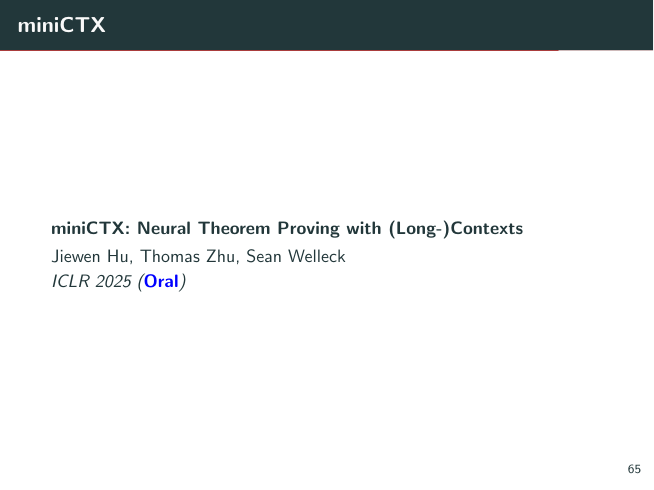
\includegraphics[width=0.80\textwidth]{figures/lec10_fig_009.png}
\caption{miniCTX 关注真实项目中的长上下文 theorem proving，而非只看局部 state 的竞赛式 proving。}
\end{figure}

其教学意义在于，它把 theorem proving 从 ``会不会走 tactic'' 推向 ``能不能在真实软件与数学项目环境中工作''。对 agent 而言，这意味着不仅要学会 reasoning，还要学会上下文管理、检索与工作记忆。

\subsection{真实项目环境中的差异}

\begin{figure}[H]
\centering
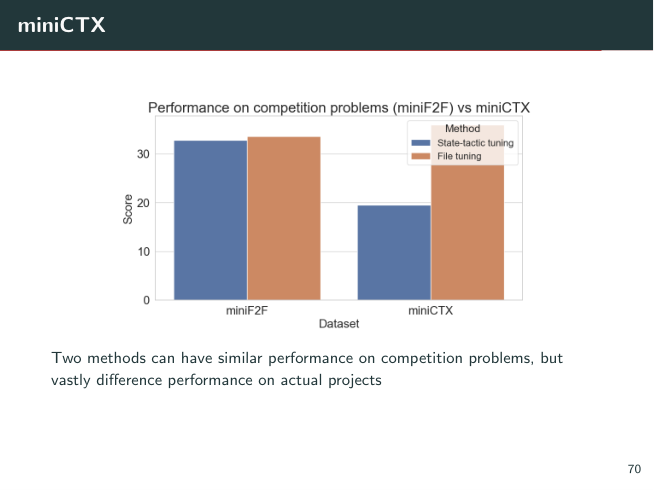
\includegraphics[width=0.80\textwidth]{figures/lec10_fig_010.png}
\caption{真实项目的长上下文会显著区分方法能力；竞赛 benchmark 上相近的方法，落到真实项目上可能差很多。}
\end{figure}

slides 特别强调了一个经常被忽略的事实：两个方法在竞赛 benchmark 上可以非常接近，但在真实项目里却可能差异巨大。原因是竞赛题通常不依赖新定义、长文件上下文与项目规范；而 research-level formalization 恰恰依赖这些。若系统只会在局部 state 上做模式匹配，它在真实项目里就会迅速失效。

\section{reading 融合、proof optimization 与课程衔接}

\subsection{四篇 readings 如何补全本讲}

Lean-STaR 说明 \emph{thinking before proving} 能提升 formal proof search；DSP 说明 \emph{informal proof sketches} 可以引导 low-level prover；miniCTX 说明 \emph{真实项目上下文} 是新的 benchmark frontier；ImProver 则补上了 \emph{proof optimization} 这一维度：agent 不仅能找到 proof，还能在 correctness 不变时优化 proof 的长度、可读性与模块化。

这四篇 reading 放在一起，可以看出一个清晰演化路径：
\begin{enumerate}
\item 先让模型在局部 state 上会走 tactic。
\item 再让模型显式地产生 thoughts，利用更多 inference-time reasoning。
\item 再让系统把 informal sketch、retrieval、context management 接入 proving。
\item 最后让 agent 不只 ``找到一个 proof''，而是能围绕 proof 做持续的搜索、重写与优化。
\end{enumerate}

\subsection{与课程前后讲的联系}

与 L08/L09 相比，这一讲更强调 theorem proving 内部的系统设计，而不是单一 benchmark 成绩。与 L01 相比，这一讲给出一个更尖锐的例子：\textbf{test-time compute 只有在 proof environment 提供 verifier 信号时，才真正变成可靠的推理改进手段。} 与下一讲关于 abstraction/discovery 的关系也很直接：一旦 theorem proving 不再只靠局部 tactic，而要利用高层 sketch、concept、context 和 project structure，abstraction 就成了下一步自然主题。

\section{本章小结}

本讲的主线可以概括成一句话：\textbf{高级 theorem proving 不只是“更强的证明模型”，而是“把 informal reasoning、formal verification、retrieval、search 和 context management 组合成可验证的 agent workflow”。} Lean-STaR 让 ``想'' 成为策略的一部分，DSP 让高层 sketch 成为低层 proving 的搜索偏置，LeanHammer 把 premise selection 与 ATP 集成为低层 automation，miniCTX 则逼着我们直面真实项目的长上下文依赖。对 LLM agent 研究者而言，这一讲的重要性在于它展示了一个极其清晰的范式：当环境能给出强反馈时，agent 才真正可以在 reasoning、search 与 self-improvement 上形成闭环。

\section{复习题}
\begin{enumerate}
\item informal mathematics 与 formal mathematics 的主要差异是什么？为什么 formal proof 更适合作为 agent 的训练或评估环境？
\item Lean-STaR 为什么要在 tactic 之前生成 thought？这一步解决了传统 neural theorem proving 的哪个缺口？
\item Draft, Sketch, Prove 中的 sketch 为什么不能被理解成 ``最终证明''？
\item hammer 系统中的 premise selection 扮演什么角色？若 premise selection 很差，会发生什么？
\item miniCTX 想解决什么 benchmark blind spot？
\end{enumerate}

\section{深入思考题}
\begin{enumerate}
\item 如果未来 frontier model 在自然语言证明上非常强，是否还需要 proof assistant 反馈？请结合 hallucination control 与 theorem proving 的要求回答。
\item 对 theorem proving 来说，thought 是不是总是越长越好？什么时候更长的 thought 反而会伤害搜索？
\item research-level formalization 与 coding agents 在系统层面有哪些共同点？
\end{enumerate}

\section{延伸阅读}
\begin{itemize}
\item Lean-STaR: Learning to Interleave Thinking and Proving
\item Draft, Sketch, and Prove: Guiding Formal Theorem Provers with Informal Proofs
\item miniCTX: Neural Theorem Proving with (Long-)Contexts
\item ImProver: Agent-Based Automated Proof Optimization
\end{itemize}

\end{document}
